% Provenance (never printed): see sources/outline_sources.md (Year 3:
% planetary atmospheres, escape, the runaway greenhouse, Mars, Titan,
% habitability).
% Brief: sources/book5/BRIEFS.md, ch. 27. Curves from figdata/bachelor-3/
% jeans_escape.py (escape parameter and escaping fraction at the exobases
% of Venus, the Earth, Mars and Titan), runaway_greenhouse.py (an
% illustrative grey model of a moist atmosphere: OLR against surface
% temperature) and habitability.py (the habitable-zone fits of Kopparapu et
% al. 2013; the phase boundaries of water and methane with the surface
% states of four bodies). Exercise and problem values in the Book 5 scratch
% calculator calc/ch27.py. Kepos and its star are invented.
\chapter{Atmosferas planetárias e habitabilidade}\label{ch:b3:planetary-atmospheres}

Vênus e a Terra são quase gêmeas: quase do mesmo tamanho, densidades médias semelhantes,
órbitas vizinhas. No entanto, Vênus mantém \qty{92}{bar} de dióxido de carbono
sobre uma superfície a \qty{737}{K}, e tem tão pouca água que, espalhada sobre a
superfície, formaria uma camada com cerca de um centímetro de profundidade. O
espectrômetro de massa da sonda Pioneer Venus, ao atravessar suas nuvens,
mediu a razão entre deutério e hidrogênio nessa água: \num{0.016}, cem vezes a
razão nos oceanos da Terra. O hidrogênio leve escapa para o espaço mais
facilmente que o deutério pesado; o que sobra de um grande reservatório
que perdeu a maior parte do seu hidrogênio é rico em deutério. A razão é o
vestígio da água que Vênus um dia teve e perdeu. Este capítulo pergunta como
um planeta retém o seu ar e a sua água, e como os perde.
% ledger: planet:Venus.diameter, planet:Earth.diameter, planet:Venus.density, planet:Earth.density, nasa:venus-atm, arney18:venus-water, donahue82:dh, kc98:standards

\begin{recall}
A altura de escala, a fórmula barométrica, a distribuição de Maxwell--Boltzmann,
a velocidade de escape, o caminho livre médio e o efeito estufa estão nos livros
de física. A zona habitável de uma estrela está nos livros do ensino médio. A
temperatura de equilíbrio e o albedo de Bond estão no volume do primeiro ano, no
seu capítulo sobre planetologia comparada; a profundidade óptica, no seu capítulo
sobre telescópios e fotometria; as taxas de variação da temperatura com a altura,
no seu capítulo sobre a estrutura da atmosfera e do oceano; a radiação de onda
longa emitida para o espaço (OLR) e a temperatura de emissão, no seu capítulo
sobre radiação e transporte de calor. O adiabático úmido está no volume do segundo
ano, no seu capítulo sobre termodinâmica atmosférica; a linha de neve, no seu
capítulo sobre formação planetária; o ciclo longo do carbono e o termostato do
intemperismo de silicatos, no seu capítulo sobre o clima ao longo do tempo
geológico. A \omterm{prop:b3:stable-isotopes:rayleigh-distillation}{destilação de Rayleigh} está neste volume, no seu capítulo sobre
isótopos estáveis.
\end{recall}

\section{A estrutura de uma atmosfera}\label{sec:b3:planetary-atmospheres:structure}

Uma atmosfera isotérmica de massa molecular $m$ à temperatura $T$ rarefaz-se
com a altura segundo $p = p_0\,e^{-z/H}$, com a altura de escala $H = kT/mg$. Na
superfície da Terra, $H$ é de cerca de \qty{8}{km}; na superfície de
Titã, onde a gravidade é fraca e o ar é frio, de cerca de \qty{20}{km}.

A temperatura, porém, não é uniforme. A luz solar que chega ao solo o aquece;
o ar acima, que absorve e emite no infravermelho, é aquecido por baixo.
A radiação, por si só, tornaria a atmosfera inferior tão íngreme em temperatura
que ela se inverteria.

\begin{definition}[Equilíbrio radiativo--convectivo]\label{def:b3:planetary-atmospheres:rce}
Uma coluna de atmosfera está em \emph{equilíbrio
radiativo--convectivo}\index{equilíbrio radiativo--convectivo} quando, em cada nível,
o fluxo líquido de radiação está equilibrado, exceto em uma camada inferior onde
a convecção transporta calor para cima e mantém o gradiente de temperatura
no adiabático. A camada inferior, convectiva, é a troposfera; a camada superior,
em equilíbrio radiativo, a estratosfera; a tropopausa é o nível onde elas se
encontram.
\end{definition}

A atmosfera mais simples em que isso pode ser acompanhado é a \emph{cinza}: ela é
transparente à luz solar e absorve igualmente todo comprimento de onda infravermelho,
com uma profundidade óptica $\tau$ contada de cima para baixo.

\begin{proposition}[Equilíbrio radiativo de uma atmosfera cinza]\label{prop:b3:planetary-atmospheres:grey}
Em uma atmosfera cinza em equilíbrio radiativo que emite o fluxo $F$ para o
espaço, a temperatura na profundidade óptica $\tau$ obedece a
\[
\sigma T^4(\tau) = \frac F2\,(1 + D\tau),
\]
onde $D \approx 1.66$ leva em conta os trajetos oblíquos da radiação.
O topo da atmosfera está na \emph{temperatura de pele}
$T_\mathrm{skin} = 2^{-1/4}\,T_e$, onde $T_e = (F/\sigma)^{1/4}$ é a
temperatura de emissão.
\end{proposition}

A proposição é admitida; ela decorre das equações de dois fluxos para
os fluxos ascendente e descendente. Onde $\tau$ é grande, perto do solo,
a temperatura radiativa varia rapidamente com $\tau$, e $\tau$ cresce
depressa com a profundidade porque o gás absorvedor é mais denso ali: o
perfil radiativo é mais íngreme que o adiabático, e a convecção assume o controle.
No alto, $\tau$ é pequeno e a temperatura tende à temperatura de pele. A Terra
emite cerca de \qty{239}{W.m^{-2}} para o espaço, com uma temperatura de
emissão de \qty{255}{K} e uma temperatura de pele de \qty{214}{K};
a atmosfera padrão situa sua tropopausa a \qty{11}{km} e \qty{216.65}{K}.
O modelo cinza, por mais grosseiro que seja, posiciona o topo frio da
troposfera aproximadamente no lugar certo.
% ledger: ipcc:budget-toa, ussa76:sea-level, ussa76:layers, const:sigma

\begin{omfigure}
\centering
\begin{tikzpicture}[x=1cm, y=0.8cm, font=\small]
% temperature profile (schematic)
\draw[->] (0,0) -- (6.8,0) node[below left, font=\scriptsize] {temperatura};
\draw[->] (0,0) -- (0,8.4) node[above, font=\scriptsize] {altura};
\draw[thick, omDef] (5.6,0) -- (4.2,2.0) -- (4.2,2.6) -- (4.7,3.6)
  -- (3.8,4.6) .. controls (4.3,5.6) and (5.9,6.0) .. (6.2,6.6) -- (6.25,8.2);
\draw[dashed, black!50] (0,2.0) -- (6.8,2.0) node[right, font=\scriptsize, black] {tropopausa};
\draw[dashed, black!50] (0,4.6) -- (6.8,4.6) node[right, font=\scriptsize, black] {homopausa};
\draw[thick, red!70!black] (0,6.6) -- (6.8,6.6) node[right, font=\scriptsize] {exobase};
\node[anchor=west, font=\scriptsize] at (0.15,0.9) {troposfera: convecção};
\node[anchor=west, font=\scriptsize] at (0.15,0.5) {(adiabático)};
\node[anchor=west, font=\scriptsize] at (0.15,3.2) {estratosfera:};
\node[anchor=west, font=\scriptsize] at (0.15,2.8) {equilíbrio radiativo};
\node[anchor=west, font=\scriptsize] at (0.15,5.6) {termosfera};
\node[anchor=west, font=\scriptsize] at (0.15,5.2) {(aquecida por EUV)};
\node[anchor=west, font=\scriptsize] at (0.15,7.6) {exosfera:};
\node[anchor=west, font=\scriptsize] at (0.15,7.2) {sem colisões};
% exosphere trajectories
\begin{scope}[shift={(11.0,0)}]
\fill[black!8] (-2.3,0) rectangle (2.3,6.6);
\draw[red!70!black, thick] (-2.3,6.6) -- (2.3,6.6);
\node[font=\scriptsize] at (0,0.5) {colisões em toda parte};
\node[font=\scriptsize, align=center] at (0,3.3) {gás misturado por\\turbulência abaixo da\\homopausa, separado\\por difusão molecular\\acima dela};
\draw[->, thick, omDef] (-1.6,6.6) .. controls (-1.4,8.0) and (-0.9,8.0) .. (-0.7,6.6);
\node[font=\scriptsize, omDef] at (-1.15,8.3) {balística};
\draw[->, thick, red!70!black] (0.4,6.6) -- (1.2,8.5);
\node[font=\scriptsize, red!70!black, anchor=west] at (1.25,8.3) {escapando};
\node[font=\scriptsize, align=center, anchor=north] at (0,6.45) {$v > v_\mathrm{esc}$ para cima:\\ perdida para o espaço};
\end{scope}
\end{tikzpicture}
\par\smallskip{\small As camadas de uma atmosfera planetária (esquemático, não
em escala). À esquerda: um perfil de temperatura semelhante ao da Terra, com a
troposfera mantida no adiabático pela convecção, uma estratosfera em
equilíbrio radiativo e uma termosfera aquecida do alto pela luz solar
ultravioleta extrema. À direita: acima da \omterm{def:b3:planetary-atmospheres:exobase}{exobase}, uma partícula não encontra
nada; uma que se move para cima mais depressa que a velocidade de escape
deixa o planeta, uma mais lenta cai de volta em um arco balístico.}\label{fig:b3:planetary-atmospheres:structure}
\end{omfigure}
% ledger: gronoff:exobase, gronoff:diffusion

Muito alto na atmosfera, o ar é tão rarefeito que uma molécula pode percorrer uma grande distância
entre colisões. Onde ela pode percorrer mais que uma altura de escala, deixa de
pertencer a um fluido.

\begin{definition}[Exobase; exosfera]\label{def:b3:planetary-atmospheres:exobase}
A \emph{exobase}\index{exobase} de uma atmosfera é o nível em que o
caminho livre médio de suas partículas iguala a altura de escala. Acima dele,
a \emph{exosfera}\index{exosfera}, uma partícula que se move para cima
dificilmente encontra outra, e uma mais rápida que a velocidade de escape local
deixa o planeta.
\end{definition}

\begin{proposition}[Condição da exobase]\label{prop:b3:planetary-atmospheres:exobase}
Em uma atmosfera isotérmica de partículas de seção de choque de colisão
$\sigma_c$, uma partícula que se move verticalmente para cima a partir do nível de densidade
$n$ escapa de todas as colisões com probabilidade $e^{-n\sigma_c H}$. Na
\omterm{def:b3:planetary-atmospheres:exobase}{exobase} $n\sigma_c H = 1$: a probabilidade é $1/e$.
\end{proposition}

\begin{proof}
Ao longo de um trajeto $\mathrm dz$, a partícula encontra, em média, $n(z)\sigma_c\,
\mathrm dz$ outras. A probabilidade de não encontrar nenhuma no trajeto para cima a
$z_0$ é $\exp(-\sigma_c\int_{z_0}^\infty n\,\mathrm dz)$, e, em uma
atmosfera isotérmica $\int_{z_0}^\infty n_0\,e^{-(z-z_0)/H}\,\mathrm dz
= n_0 H$. O caminho livre médio é $\ell = 1/n\sigma_c$; a condição $\ell
= H$ equivale a $n\sigma_c H = 1$.
\end{proof}

A \omterm{def:b3:planetary-atmospheres:exobase}{exobase} situa-se a cerca de \qty{500}{km} na Terra, \qty{200}{km} em
Vênus e em Marte, e perto de \qty{1500}{km} em Titã, mais da metade do
raio da lua.
% ledger: gronoff:exobases

\section{Escape atmosférico}\label{sec:b3:planetary-atmospheres:escape}

Na \omterm{def:b3:planetary-atmospheres:exobase}{exobase}, as partículas mantêm a distribuição de Maxwell--Boltzmann de
velocidades do gás abaixo. Sua cauda sempre contém algumas partículas mais rápidas que
a velocidade de escape.

\begin{definition}[Escape de Jeans; parâmetro de escape]\label{def:b3:planetary-atmospheres:jeans-escape}
O \emph{escape de Jeans}\index{escape de Jeans} é a perda para o espaço das
partículas da cauda de Maxwell--Boltzmann que, na \omterm{def:b3:planetary-atmospheres:exobase}{exobase}, se movem para cima
mais depressa que a velocidade de escape. O \emph{parâmetro de
escape}\index{parâmetro de escape} de partículas de massa $m$ na \omterm{def:b3:planetary-atmospheres:exobase}{exobase},
de raio $r$ e temperatura $T$, em um planeta de massa $M$, é
\[
\lambda = \frac{GMm}{kTr} = \frac{v_\mathrm{esc}^2}{u^2},
\qquad u = \sqrt{\frac{2kT}m},
\]
a razão entre sua energia de ligação gravitacional e $kT$, e também o
quadrado da velocidade de escape dividido pela velocidade térmica mais provável $u$.
\end{definition}

\begin{theorem}[Fluxo de Jeans]\label{thm:b3:planetary-atmospheres:jeans}
Em uma \omterm{def:b3:planetary-atmospheres:exobase}{exobase} de densidade $n$, o número de partículas que escapam por unidade
de área e por unidade de tempo é
\[
\Phi_\mathrm J = \frac{n\,u}{2\sqrt\pi}\,(1 + \lambda)\,e^{-\lambda}.
\]
\end{theorem}

\begin{proof}
A distribuição de Maxwell--Boltzmann das velocidades é $f(\vec v) =
n\,(\pi u^2)^{-3/2}\,e^{-v^2/u^2}$. Uma partícula de velocidade $v$ que se move
com ângulo $\theta$ em relação à vertical atravessa uma área horizontal unitária à
taxa $v\cos\theta$. Contando apenas as velocidades para cima ($0 \le \theta \le
\pi/2$) mais rápidas que $v_\mathrm{esc}$,
\[
\Phi_\mathrm J = \frac{n}{\pi^{3/2}u^3}\int_0^{2\pi}\!\!\mathrm d\varphi
\int_0^{\pi/2}\!\!\cos\theta\sin\theta\,\mathrm d\theta
\int_{v_\mathrm{esc}}^\infty v^3e^{-v^2/u^2}\,\mathrm dv
= \frac{n}{\pi^{3/2}u^3}\cdot2\pi\cdot\frac12\cdot
\frac{u^4}2\,(1 + \lambda)\,e^{-\lambda},
\]
onde a última integral segue da substituição $s = v^2/u^2$ e de
uma integração por partes: $\int_\lambda^\infty s\,e^{-s}\,\mathrm ds =
(1 + \lambda)e^{-\lambda}$. Reunindo os termos, $\Phi_\mathrm J = n u (1 +
\lambda) e^{-\lambda}/(2\sqrt\pi)$.
\end{proof}

O fator $n u/2\sqrt\pi$ é o fluxo de todas as partículas que atravessam a
\omterm{def:b3:planetary-atmospheres:exobase}{exobase} para cima; $(1 + \lambda)e^{-\lambda}$ é a fração delas
que escapam. Ela cai exponencialmente com a massa da partícula, pois
$\lambda \propto m$. Na \omterm{def:b3:planetary-atmospheres:exobase}{exobase} da Terra, a \qty{1000}{K}, o hidrogênio
tem $\lambda = 7.0$ e escapa à taxa de 0.7\,\% de seu fluxo para cima;
o deutério, $\lambda = 14$, à taxa de \num{1.2e-5}; o hélio, $\lambda = 28$,
à taxa de \num{2e-11}; o oxigênio, $\lambda = 111$, não escapa de modo algum. Na \omterm{def:b3:planetary-atmospheres:exobase}{exobase}
de Vênus, mais fria e igualmente profunda no poço gravitacional, $\lambda = 22$ mesmo para
o hidrogênio; em Marte $\lambda = 5.4$; em Titã $\lambda = 1.5$ para o hidrogênio
e 3.0 para o hidrogênio molecular.
% ledger: gronoff:jeans, gronoff:jeans-table, gronoff:exobases

\begin{omfigure}
\centering
\begin{tikzpicture}
\begin{axis}[name=lam, width=0.47\linewidth, height=0.46\linewidth,
  xmin=0.5, xmax=50, ymin=0.5, ymax=2000, xmode=log, ymode=log,
  xlabel={massa da partícula (u)}, ylabel={parâmetro de escape $\lambda$},
  tick label style={font=\scriptsize}, label style={font=\small},
  xtick={1,2,4,16,28,44}, xticklabels={1,2,4,16,28,44},
  title={(a)}, title style={font=\small},
  legend style={font=\scriptsize, at={(0.5,-0.24)}, anchor=north, legend columns=2, draw=none}]
\fill[black!10] (axis cs:0.5,0.5) rectangle (axis cs:50,2.5);
\node[font=\scriptsize, anchor=east] at (axis cs:40,1.0) {hidrodinâmico};
\addplot[thick, orange!80!black] table[x=A, y=Venus] {figdata/out/bachelor-3-jeans_escape-lambda.dat};
\addlegendentry{Vênus}
\addplot[thick, omDef] table[x=A, y=Earth] {figdata/out/bachelor-3-jeans_escape-lambda.dat};
\addlegendentry{Terra}
\addplot[thin, omDef, dashed, forget plot] table[x=A, y=EarthLo] {figdata/out/bachelor-3-jeans_escape-lambda.dat};
\addplot[thin, omDef, dashed, forget plot] table[x=A, y=EarthHi] {figdata/out/bachelor-3-jeans_escape-lambda.dat};
\addplot[thick, red!70!black] table[x=A, y=Mars] {figdata/out/bachelor-3-jeans_escape-lambda.dat};
\addlegendentry{Marte}
\addplot[thick, black!60] table[x=A, y=Titan] {figdata/out/bachelor-3-jeans_escape-lambda.dat};
\addlegendentry{Titã}
\end{axis}
\begin{axis}[at={(lam.east)}, anchor=west, xshift=0.1\linewidth,
  width=0.47\linewidth, height=0.46\linewidth,
  xmin=0, xmax=40, ymin=1e-16, ymax=1, ymode=log,
  xlabel={parâmetro de escape $\lambda$}, ylabel={fração que escapa},
  ytick={1e-16,1e-12,1e-8,1e-4,1},
  tick label style={font=\scriptsize}, label style={font=\small},
  title={(b)}, title style={font=\small}]
\addplot[thick, black] table[x=lam, y=f] {figdata/out/bachelor-3-jeans_escape-factor.dat};
\addplot[only marks, mark=*, mark size=1.8pt, omDef] table[x=lambdaEarth, y=fEarth] {figdata/out/bachelor-3-jeans_escape-species.dat};
\node[font=\scriptsize, omDef, anchor=south west] at (axis cs:7.0,7.1e-3) {H};
\node[font=\scriptsize, omDef, anchor=south west] at (axis cs:14.0,1.2e-5) {D};
\node[font=\scriptsize, omDef, anchor=south west] at (axis cs:27.9,2.2e-11) {He};
\end{axis}
\end{tikzpicture}
\par\smallskip{\small (a)~O \omterm{def:b3:planetary-atmospheres:jeans-escape}{parâmetro de escape} na \omterm{def:b3:planetary-atmospheres:exobase}{exobase} em função da
massa da partícula, para Vênus (\qty{290}{K}), a Terra (\qty{1000}{K};
tracejado: 800 e \qty{1600}{K}, a faixa do ciclo solar), Marte
(\qty{270}{K}) e Titã (\qty{180}{K}); abaixo de $\lambda \approx 2.5$
(sombreado) o escape torna-se hidrodinâmico. (b)~A fração $(1 +
\lambda)e^{-\lambda}$ do fluxo para cima que escapa, com hidrogênio,
deutério e hélio na \omterm{def:b3:planetary-atmospheres:exobase}{exobase} da Terra; o oxigênio, com $\lambda = 111$,
está muito fora da escala.}\label{fig:b3:planetary-atmospheres:jeans}
\end{omfigure}
% ledger: gronoff:jeans-table, gronoff:exobases, gronoff:jeans, nasa:venus, planet:Earth.mass, nasa:mars, nasa:titan, const:G, const:kB

Quando $\lambda$ cai para alguns poucos, a imagem de partículas que escapam uma a uma
de uma atmosfera estática deixa de valer: a alta atmosfera se expande e escoa
para longe como um vento. Os modelos situam a transição em $\lambda$ entre cerca de 1.5
e 3.

\begin{definition}[Escape hidrodinâmico, não térmico e limitado por difusão]\label{def:b3:planetary-atmospheres:hydrodynamic}
O \emph{escape hidrodinâmico}\index{escape hidrodinâmico} é a perda de uma
alta atmosfera que escoa como um todo, aquecida por cima, quando seu
\omterm{def:b3:planetary-atmospheres:jeans-escape}{parâmetro de escape} é pequeno; o escoamento pode arrastar consigo partículas mais pesadas.
O \emph{escape não térmico}\index{escape não térmico} é a perda de
partículas aceleradas por processos que não o calor: reações fotoquímicas
que dão aos fragmentos mais do que a energia de escape, íons capturados
pelo campo elétrico do vento solar, pulverização por íons que atingem
a alta atmosfera e o escoamento de íons ao longo das linhas do campo magnético.
O \emph{escape limitado por difusão}\index{escape limitado por difusão} é o escape
cuja taxa não é fixada na \omterm{def:b3:planetary-atmospheres:exobase}{exobase}, mas mais abaixo, pela velocidade com que
o gás que escapa consegue difundir-se para cima através do gás mais pesado acima da
\emph{homopausa}\index{homopausa}, o nível acima do qual a difusão molecular,
e não a turbulência, controla a mistura.
\end{definition}
% ledger: gronoff:jeans, gronoff:nonthermal, gronoff:diffusion

\begin{proposition}[Limite de difusão]\label{prop:b3:planetary-atmospheres:diffusion}
Um gás leve de razão de mistura $f$ e massa molecular $m_i$, difundindo-se
através de um gás mais pesado de massa molecular $m_a$ e altura de escala $H_a =
kT/m_a g$ com o parâmetro de difusão binária $b$, não pode subir mais rápido
do que
\[
\Phi_\mathrm{DL} = b\,f\left(\frac1{H_a} - \frac1{H_i}\right)
= \frac{b\,f\,(m_a - m_i)\,g}{kT} \approx \frac{b\,f}{H_a}.
\]
\end{proposition}

\begin{proof}
A teoria cinética (admitida) fornece o fluxo ascendente do gás leve
em relação ao gás pesado, em uma coluna isotérmica, como $\Phi = -b\,f\,
[\,(1/f)\,\mathrm df/\mathrm dz + 1/H_i - 1/H_a\,]$: o gás leve
difunde-se para baixo seguindo seu próprio gradiente, e sua altura de escala $H_i$ é maior
do que $H_a$. O fluxo é máximo quando a razão de mistura é uniforme, $\mathrm
df/\mathrm dz = 0$; o gás que escapa não pode ser retirado mais depressa sem que sua
razão de mistura caia com a altura. Com $1/H = mg/kT$, as duas
formas decorrem.
\end{proof}

Para o hidrogênio molecular subindo através do dióxido de carbono, $b \approx
\qty{1.2e19}{cm^{-1}.s^{-1}}$ a \qty{200}{K}, e, com a gravidade da Terra,
o limite é $\Phi_\mathrm{DL} \approx
\num{3.0e13}\,f\,(\qty{200}{K}/T)^{1/4}$ moléculas de $\ce{H2}$ por
centímetro quadrado e por segundo, $f$ contando todo o hidrogênio como $\ce{H2}$. Na
Terra de hoje o escape de hidrogênio é limitado por difusão: no mínimo solar,
quando a \omterm{def:b3:planetary-atmospheres:exobase}{exobase} é mais fria e o \omterm{def:b3:planetary-atmospheres:jeans-escape}{escape de Jeans} mais lento, o escape por troca
de carga com íons compensa a diferença, e o total permanece aproximadamente
o mesmo. O suprimento, e não a
\omterm{def:b3:planetary-atmospheres:exobase}{exobase}, define a taxa.
% ledger: zahnle19:diffusion, gronoff:diffusion, gronoff:rates

\section{Vênus e a estufa descontrolada}\label{sec:b3:planetary-atmospheres:venus}

Vênus recebe \qty{2601}{W.m^{-2}} do Sol, 1.91 vezes a parcela da Terra.
Suas nuvens de ácido sulfúrico refletem 77\,\% dela, de modo que absorve
menos do que a Terra; no entanto sua superfície está a \qty{737}{K} sob \qty{92}{bar}
de uma atmosfera com 96.5\,\% de dióxido de carbono. Ela contém \qty{6e15}{kg} de água,
contra \qty{1.4e21}{kg} na Terra, cerca de 30 partes por milhão em
volume abaixo das nuvens.
% ledger: nasa:venus, nasa:venus-atm, arney18:venus-water

Um planeta com oceano é mantido em equilíbrio pela sua radiação emergente. Se
ele aquece, evapora mais água; o vapor de água é um gás de efeito estufa, de modo que a
radiação emergente cresce menos do que $\sigma T^4$, mas cresce, e o
aquecimento para. Existe um limite para esse crescimento.

\begin{proposition}[Limite de radiação de uma atmosfera úmida]\label{prop:b3:planetary-atmospheres:limit}
Quando a superfície de um planeta com oceano está quente o bastante para que o vapor de água
domine sua alta atmosfera, a temperatura ali segue a
curva de saturação da água, e a radiação infravermelha para o espaço provém de
um nível de pressão fixa. Sua temperatura e a radiação emergente
deixam de crescer com a temperatura da superfície.
\end{proposition}

\begin{proof}
Em uma coluna saturada e dominada pelo vapor, a pressão $p$ em cada
nível é a pressão de saturação na temperatura local, $p =
p_\mathrm{sat}(T)$. A radiação para o espaço sai de uma região em torno do nível
onde a profundidade óptica a partir do topo vale cerca de um. Para um gás cinzento de
coeficiente de absorção de massa $\kappa$, a profundidade óptica acima da pressão $p$
é $D\kappa p/g$, de modo que esse nível fica em $p_1 = g/D\kappa$, qualquer que seja a
temperatura da superfície, e sua temperatura é aquela em que
$p_\mathrm{sat}(T) = p_1$. O aquecimento da superfície apenas acrescenta vapor abaixo dele.
\end{proof}

\begin{definition}[Estufa descontrolada; limite de estufa descontrolada; estufa úmida]\label{def:b3:planetary-atmospheres:runaway}
O \emph{limite de estufa descontrolada}\index{limite de estufa descontrolada} é o
maior fluxo de radiação infravermelha que um planeta com oceano pode enviar ao
espaço. Uma \emph{estufa descontrolada}\index{estufa descontrolada} é o estado
de um planeta que absorve mais luz solar do que esse limite: ele não consegue equilibrar
seu balanço até que todo o oceano tenha evaporado e a superfície tenha
aquecido muito além dele. Uma \emph{estufa úmida}\index{estufa úmida}
é o estado de um planeta, aquém da estufa descontrolada, cuja superfície é quente o bastante
para que sua estratosfera contenha uma grande razão de mistura de vapor de água,
que a luz ultravioleta decompõe, e cujo hidrogênio escapa.
\end{definition}

Modelos simples, como o da proposição, fornecem tal limite; com as linhas reais
do vapor de água, um cálculo linha por linha sem nuvens coloca-o em
\qty{291}{W.m^{-2}} para um planeta semelhante à Terra, e
as revisões citam cerca de \qty{300}{W.m^{-2}}. Acima de cerca de \qty{2000}{K} o
fluxo emergente volta a crescer, pois a atmosfera inferior quente irradia no
visível e no infravermelho próximo, onde a água absorve pouco: um planeta
em \omterm{def:b3:planetary-atmospheres:runaway}{estufa descontrolada} se estabiliza em uma temperatura muito alta, quando seu oceano
está todo na forma de vapor.
% ledger: kopparapu13:runaway, arney18:runaway

\begin{omfigure}
\centering
\begin{tikzpicture}
\begin{axis}[width=0.8\linewidth, height=0.48\linewidth,
  xmin=250, xmax=600, ymin=150, ymax=560,
  xlabel={temperatura da superfície (\unit{K})},
  ylabel={fluxo (\unit{W.m^{-2}})},
  tick label style={font=\scriptsize}, label style={font=\small}]
\addplot[very thick, omDef] table[x=Ts, y=olr] {figdata/out/bachelor-3-runaway_greenhouse-olr.dat};
\addplot[dashed, black!60, domain=250:600] {291};
\addplot[thick, orange!80!black, domain=250:600] {525};
\addplot[thick, orange!60!black, densely dotted, domain=250:600] {367};
\addplot[thick, black!70, densely dashed, domain=250:600] {238};
\node[font=\scriptsize, black!60, anchor=south east] at (axis cs:595,291) {limite linha a linha, \qty{291}{W.m^{-2}}};
\node[font=\scriptsize, orange!80!black, anchor=south east] at (axis cs:595,525) {Vênus hoje, sem nuvens};
\node[font=\scriptsize, orange!60!black, anchor=south east] at (axis cs:595,367) {Vênus jovem, Sol a 70\,\%};
\node[font=\scriptsize, black!70, anchor=north east] at (axis cs:595,236) {a Terra hoje};
\node[font=\scriptsize, omDef, anchor=west] at (axis cs:264,212) {radiação emergente (modelo)};
\end{axis}
\end{tikzpicture}
\par\smallskip{\small Radiação infravermelha emergente de um planeta oceânico
semelhante à Terra, em função de sua temperatura superficial, em um modelo cinza
ilustrativo (uma adiabática úmida saturada sobre 1~bar de nitrogênio, uma estratosfera a
\qty{200}{K}, vapor de água como único absorvedor; seu coeficiente de absorção,
alargado pela pressão, é escolhido para coincidir com o limite linha a linha).
Linhas horizontais: luz solar absorvida por Vênus hoje e por um Vênus jovem
com albedo de 0.193, o albedo de uma atmosfera quente de vapor sem nuvens,
e pela Terra hoje, com seu albedo de 0.3. Onde o fluxo absorvido
fica acima do platô, nenhuma temperatura superficial o equilibra: a
\omterm{def:b3:planetary-atmospheres:runaway}{estufa descontrolada}.}\label{fig:b3:planetary-atmospheres:runaway}
\end{omfigure}
% ledger: kopparapu13:runaway, iapws:vapour-pressure, iapws4:sublimation, const:R, const:sigma, nasa:venus, gough81:luminosity, ipcc:budget-toa

Com o albedo de uma atmosfera de vapor sem nuvens, 0.193, um planeta semelhante à Terra
em torno do Sol entra em \omterm{def:b3:planetary-atmospheres:runaway}{estufa descontrolada} quando recebe 1.06 vezes a
insolação da Terra, a \qty{0.97}{au}. Antes, a 1.015 vezes a insolação da Terra
e temperatura superficial de \qty{340}{K}, sua estratosfera fica úmida:
hoje a água é retida na armadilha de frio da tropopausa, perto de
\qty{0.1}{bar}, mas em um planeta mais quente a armadilha de frio sobe e deixa o vapor
passar. Quando a razão de mistura da água na estratosfera atinge cerca de
\num{3e-3}, o \omterm{def:b3:planetary-atmospheres:hydrodynamic}{escape limitado por difusão} remove um oceano de hidrogênio em aproximadamente
a idade da Terra.
% ledger: kopparapu13:runaway, kopparapu13:water-loss, arney18:runaway

O deutério de Vênus mede o que foi perdido. Cada átomo que escapa
remove hidrogênio e um pouco de deutério do reservatório restante, assim como
cada gota que precipita remove um pouco dos isótopos pesados de uma
nuvem.

\begin{proposition}[Enriquecimento isotópico por escape]\label{prop:b3:planetary-atmospheres:dh}
Suponha-se que um reservatório de água perca hidrogênio para o espaço, escapando cada átomo de deutério
com eficiência $\alpha$ em relação a um átomo de hidrogênio
($\alpha < 1$). Quando o reservatório encolhe de $M_0$ para $M$, sua razão
$R = \mathrm{D}/\mathrm{H}$ cresce de $R_0$ para
\[
\frac R{R_0} = \left(\frac{M_0}M\right)^{1-\alpha}.
\]
\end{proposition}

\begin{proof}
Perder $\mathrm dN_\mathrm H$ átomos de hidrogênio custa ao reservatório
$\mathrm dN_\mathrm D = \alpha R\,\mathrm dN_\mathrm H$ átomos de deutério:
$\mathrm dN_\mathrm D/N_\mathrm D = \alpha\,\mathrm dN_\mathrm H/
N_\mathrm H$, logo $N_\mathrm D \propto N_\mathrm H^\alpha$ e $R \propto
N_\mathrm H^{\alpha - 1}$. A massa de água é proporcional a
$N_\mathrm H$. Trata-se da \omterm{prop:b3:stable-isotopes:rayleigh-distillation}{destilação de Rayleigh}, com o escape no lugar da
chuva.
\end{proof}

Se nenhum deutério tivesse escapado ($\alpha = 0$), um enriquecimento de cem vezes
significaria que Vênus já teve pelo menos cem vezes sua água atual.
Um escape que fraciona menos exige muito mais: no \omterm{def:b3:planetary-atmospheres:hydrodynamic}{escape limitado por difusão}
$\alpha \approx 0.8$, e um enriquecimento de cem vezes exigiria
que o reservatório encolhesse por um fator de $100^5$. A razão é lida como um
limite inferior: pelo menos alguns décimos por cento de um oceano terrestre,
e as estimativas para um oceano primitivo de Vênus vão de 4 a \qty{525}{m} distribuídos
sobre sua superfície. Restam duas ressalvas. A maior parte do fracionamento pode ter
ocorrido apenas na perda dos últimos poucos bar de água, e um suprimento constante
de água proveniente de cometas ou vulcões, perdido tão rápido quanto chegava, poderia
construir a mesma razão. Vênus ainda está perdendo água: seus íons que escapam são
hidrogênio e oxigênio na razão de dois para um, arrastados por um campo elétrico
cinco vezes mais intenso que o da ionosfera terrestre, em torno de um
planeta sem campo magnético.
% ledger: donahue82:dh, arney18:venus-water, arney18:runaway, arney18:venus-loss, zahnle19:rayleigh

\section{Marte: uma atmosfera tênue e um passado úmido}\label{sec:b3:planetary-atmospheres:mars}

Marte mantém uma pressão superficial média de \qty{6.36}{mbar}, entre 4.0 e
\qty{8.7}{mbar} ao longo das estações, 95\,\% de dióxido de carbono, a cerca de
\qty{214}{K}. A pressão mal supera a pressão do ponto triplo da
água, \qty{6.1}{mbar}: a água líquida não pode durar em sua superfície, onde
o gelo sublima. No entanto, terrenos antigos são cortados por vales ramificados, e
carregam minerais que se formam apenas em água líquida.
% ledger: nasa:mars-atm, iapws:triple-critical, nasa:mars-water, lasp:maven

\begin{omfigure}
\centering
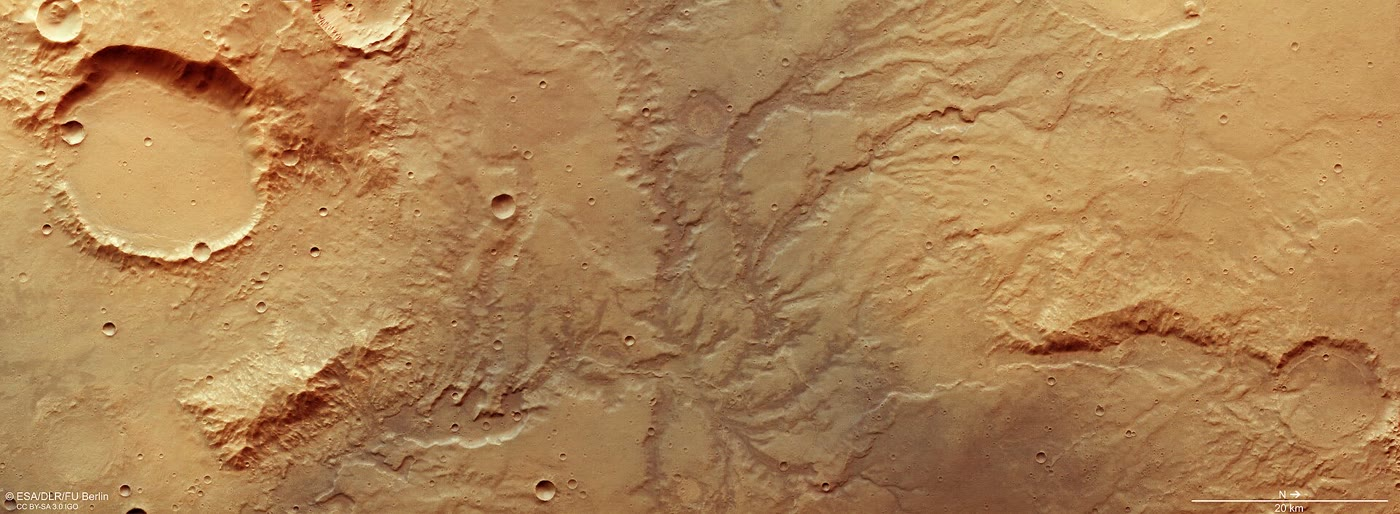
\includegraphics[width=\linewidth]{images/book5/b3-mars-valley-network.jpg}
\par\smallskip{\small Uma rede de vales secos em Marte, vista pela
câmera da Mars Express a cerca de \qty{14}{m} por pixel, perto de \ang{17}\,S,
\ang{66}\,L; o norte fica à direita, e a barra de escala tem \qty{20}{km}.
Os afluentes se unem a jusante em vales maiores, o padrão de uma
rede de drenagem. Imagem ESA/DLR/FU Berlin, CC BY-SA 3.0 IGO.}\label{fig:b3:planetary-atmospheres:valleys}
\end{omfigure}
% ledger: photo:b3-mars-valley-network

Os vales e os canais de escoamento de Marte exigem, segundo estimativas geológicas,
uma camada global de água com 100 a \qty{1500}{m} de profundidade, contra 3 a
\qty{25}{m} no gelo e no ar de hoje. Grande parte do restante foi para o espaço.
A sonda orbital MAVEN mediu o vento solar arrastando gás de Marte a cerca de
\qty{100}{g} por segundo, três quartos dele pela cauda
atrás do planeta, onde o vento solar flui, e um quarto em uma pluma
sobre os polos; durante as
tempestades solares de março de 2015, a perda se acelerou, e provavelmente foi muito
mais rápida quando o Sol jovem era mais ativo. Marte também perde hidrogênio, cerca de
\num{3e26} átomos por segundo em média hoje: mantida por quatro bilhões
de anos, uma perda equivalente a uma camada global de água de apenas cerca de \qty{4}{m} de profundidade.
% ledger: gilli25:h-loss, lasp:maven

A taxa nem sempre foi a de hoje. A obliquidade de Marte, \ang{25.2}
atualmente, oscilou entre 0 e \ang{66} nos últimos 250 milhões de anos,
em torno de uma média próxima de \ang{35}, enquanto a da Terra varia em pouco mais de um
grau. O movimento é caótico e não pode ser rastreado por bilhões de
anos; crateras elípticas formadas por impactos rasantes, cujas orientações
registram a obliquidade, sugerem uma média entre cerca de 10 e \ang{30} nos
últimos 3.5 bilhões de anos, aproximadamente. Com alta obliquidade, o polo de verão aquece,
mais vapor de água sobe, e os modelos climáticos fazem a perda de hidrogênio
vinte vezes mais rápida: ao longo da história de Marte, uma camada da ordem de
\qty{80}{m}.
% ledger: planet:Mars.obliq, gilli25:obliquity, holo18:obliquity, gilli25:h-loss

\section{Titã: um ciclo de metano}\label{sec:b3:planetary-atmospheres:titan}

Titã, uma lua menor que Marte, tem atmosfera mais espessa que a da Terra:
uma pressão na superfície cerca de 60\,\% maior, a \qty{-179}{\degreeCelsius}.
A atmosfera é composta por cerca de 95\,\% de nitrogênio e 5\,\% de metano, e, como a
gravidade da lua é fraca, a atmosfera se estende dez vezes mais alta que a da Terra, até
quase \qty{600}{km}. A luz ultravioleta separa o metano e o nitrogênio
no alto; os fragmentos se recombinam numa névoa alaranjada de hidrocarbonetos mais pesados
que oculta a superfície da luz visível. Abaixo da névoa,
o metano desempenha o papel da água: condensa-se em nuvens, chove, escava
canais de rios e enche lagos e mares de metano e etano.
% ledger: nasa:titan-surface, nasa:titan-facts

\begin{omfigure}
\centering
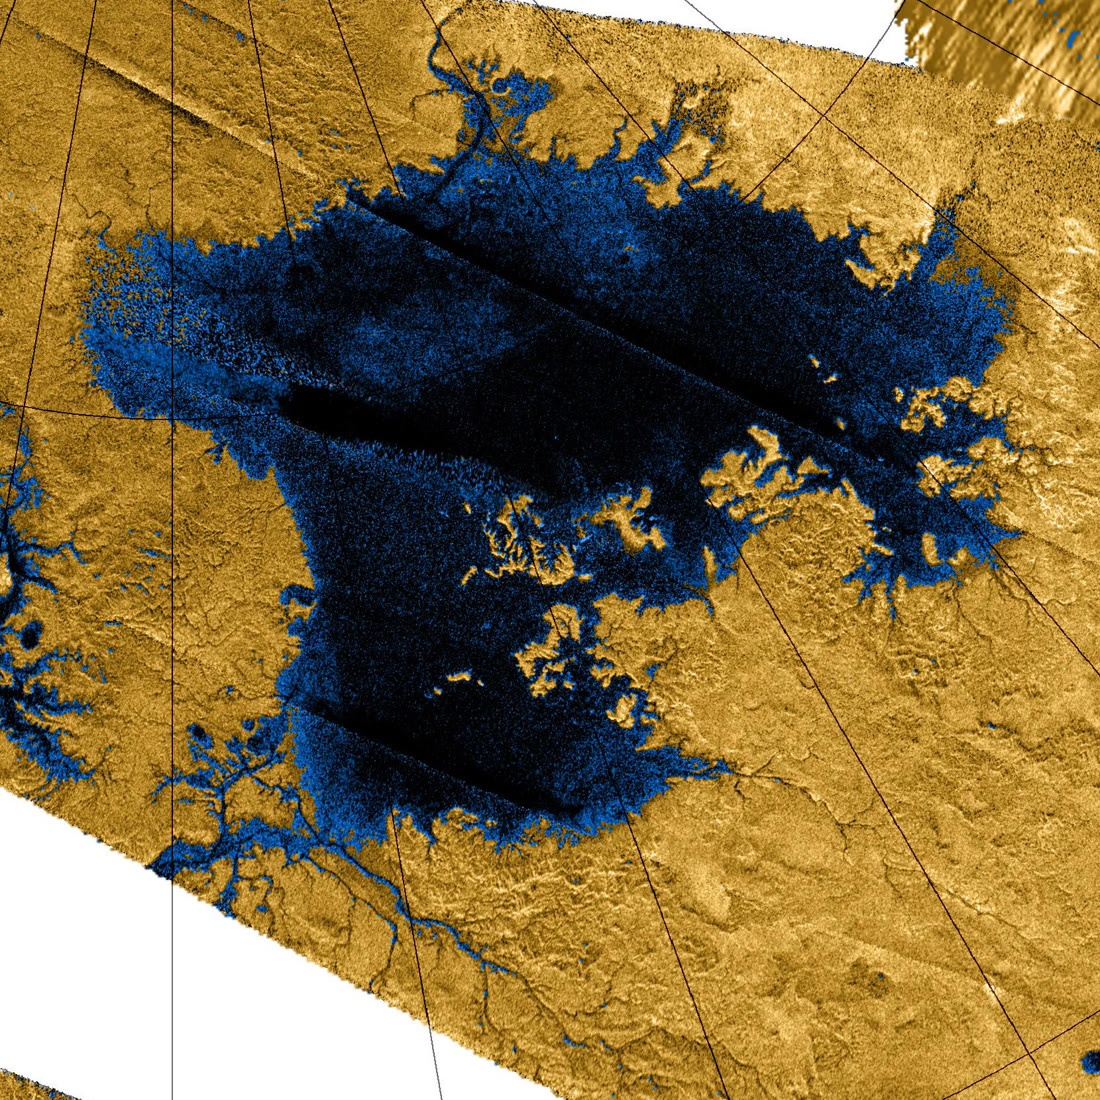
\includegraphics[width=0.5\linewidth]{images/book5/b3-ligeia-mare.jpg}
\par\smallskip{\small Ligeia Mare, um mar próximo ao polo norte de Titã, em um
mosaico de imagens de radar da Cassini em falsa cor: feições que se acredita serem
líquidas em azul e preto, terreno sólido em tom marrom, com baías, ilhas
e supostas redes tributárias. Dos cerca de 400 lagos e mares no norte mapeado,
aqueles maiores que \qty{26000}{km^2} concentram 70\,\% da área.
NASA/JPL/USGS, domínio público.}\label{fig:b3:planetary-atmospheres:ligeia}
\end{omfigure}
% ledger: photo:b3-ligeia-mare

Se um líquido pode existir sobre uma superfície depende de seu diagrama de fases e da
pressão e da temperatura ali. A superfície de Titã situa-se logo acima do
ponto triplo do metano, \qty{90.67}{K} e \qty{0.117}{bar}, e abaixo do
seu ponto crítico: metano líquido é possível, e metano a 5\,\% de
\qty{1.6}{bar} não está longe da saturação. A superfície de Marte situa-se perto do
ponto triplo da água, a da Terra bem dentro de seu campo líquido, e
a de Vênus acima da temperatura crítica da água, \qty{647}{K}, onde nenhum
líquido pode existir de maneira alguma.
% ledger: nist:methane-phase, iapws:triple-critical, nasa:titan-surface

\begin{omfigure}
\centering
\begin{tikzpicture}
\begin{axis}[width=0.8\linewidth, height=0.52\linewidth,
  xmin=60, xmax=800, ymin=1e-4, ymax=1000, ymode=log,
  xlabel={temperatura (\unit{K})}, ylabel={pressão (\unit{bar})},
  tick label style={font=\scriptsize}, label style={font=\small}]
\addplot[thick, omDef] table[x=T, y=p_bar] {figdata/out/bachelor-3-habitability-water.dat};
\addplot[thick, omDef, dashed] table[x=T, y=p_bar] {figdata/out/bachelor-3-habitability-ice.dat};
\addplot[thick, orange!80!black] table[x=T, y=p_bar] {figdata/out/bachelor-3-habitability-methane.dat};
\addplot[only marks, mark=*, mark size=1.6pt, omDef] coordinates {(273.16,0.00611657) (647.096,220.64)};
\addplot[only marks, mark=*, mark size=1.6pt, orange!80!black] coordinates {(90.67,0.1169) (190.6,46.1)};
\addplot[only marks, mark=square*, mark size=2.2pt, black] table[x=T, y=p_bar] {figdata/out/bachelor-3-habitability-bodies.dat};
\node[font=\scriptsize, anchor=south] at (axis cs:737,110) {Vênus};
\node[font=\scriptsize, anchor=west] at (axis cs:300,1.0) {Terra};
\node[font=\scriptsize, anchor=north] at (axis cs:214,0.0045) {Marte};
\node[font=\scriptsize, anchor=south] at (axis cs:94,2.2) {Titã};
\node[font=\scriptsize, omDef, anchor=west] at (axis cs:420,3) {água: líquida acima, vapor abaixo};
\node[font=\scriptsize, omDef, anchor=north west] at (axis cs:205,0.0012) {gelo};
\node[font=\scriptsize, orange!80!black, anchor=west] at (axis cs:196,46) {metano};
\node[font=\scriptsize, omDef, anchor=south east] at (axis cs:640,230) {ponto crítico};
\end{axis}
\end{tikzpicture}
\par\smallskip{\small As fronteiras entre vapor e água condensada
(azul: líquido--vapor, do ponto triplo ao ponto crítico;
tracejada: gelo--vapor) e entre o metano líquido e seu vapor (laranja),
com os estados médios da superfície de Vênus, da Terra, de Marte e de Titã
(quadrados). Um líquido pode existir sobre uma superfície cuja pressão está acima da
curva desse líquido, entre as temperaturas do seu ponto triplo e do
ponto crítico.}\label{fig:b3:planetary-atmospheres:phases}
\end{omfigure}
% ledger: iapws:vapour-pressure, iapws4:sublimation, iapws:triple-critical, nist:methane-phase, nasa:venus-atm, planet:Earth.Tmean, planet:Earth.psurf, nasa:mars-atm, nasa:titan-surface

Titã retém seu nitrogênio com facilidade: na sua \omterm{def:b3:planetary-atmospheres:exobase}{exobase} $\lambda = 41$ para
nitrogênio. Seu hidrogênio, com $\lambda$ próximo de 1.5, escapa quase livremente, e
o escape do hidrogênio molecular é fixado mais abaixo pelo fluxo limitante
através da \omterm{def:b3:planetary-atmospheres:hydrodynamic}{homopausa}, como na Terra. Os compostos pesados formados a partir do
metano quebrado sedimentam-se na superfície, onde formam a areia de vastos
campos de dunas.
% ledger: gronoff:jeans-table, gronoff:diffusion, nasa:titan-surface

\section{Habitabilidade planetária}\label{sec:b3:planetary-atmospheres:habitability}

A zona habitável dos livros escolares é a faixa de distâncias a partir de uma
estrela na qual um planeta como a Terra pode manter água líquida em sua
superfície. Suas bordas são os limites vistos neste capítulo.

\begin{definition}[Habitabilidade planetária]\label{def:b3:planetary-atmospheres:habitability}
A \emph{habitabilidade planetária}\index{habitabilidade planetária} de um
planeta é sua capacidade de manter água líquida na superfície ao longo de
tempos geológicos: recebe um fluxo estelar dentro dos limites da
zona habitável, retém sua atmosfera e sua água contra o
escape, e um ciclo de carbono de longo prazo regula seu clima.
\end{definition}

A borda interna da zona habitável é a \omterm{def:b3:planetary-atmospheres:runaway}{estufa úmida} ou a \omterm{def:b3:planetary-atmospheres:runaway}{estufa
descontrolada}: um planeta semelhante à Terra ao redor do Sol torna-se úmido a
\qty{0.99}{au} e atinge a \omterm{def:b3:planetary-atmospheres:runaway}{estufa descontrolada} a \qty{0.97}{au}. A borda externa é a
\emph{estufa máxima}: a adição de dióxido de carbono aquece um planeta apenas até
o gás extra espalha de volta mais luz solar do que o seu efeito estufa
ganha; ao redor do Sol isso ocorre a
\qty{1.70}{au}, sob cerca de \qty{8}{bar} de dióxido de carbono. Essas são
bordas conservadoras, calculadas sem nuvens. Duas bordas empíricas são mais amplas:
Vênus parece não ter tido água superficial por pelo menos um bilhão de anos,
quando recebeu 1.76 vezes a luz solar atual da Terra (\qty{0.75}{au});
Marte teve água corrente quando recebeu 0.32 vez essa luz solar, se seus
vales têm 3.8 bilhões de anos (\qty{1.77}{au}). Em torno de estrelas mais frias, os mesmos limites ocorrem
em fluxos mais baixos, porque sua luz mais avermelhada é espalhada menos e absorvida
mais pela água e pelo dióxido de carbono.
% ledger: kopparapu13:runaway, kopparapu13:outer, kopparapu13:hz-fit

\begin{omfigure}
\centering
\begin{tikzpicture}
\begin{axis}[width=0.8\linewidth, height=0.5\linewidth,
  xmin=0, xmax=2.1, ymin=2600, ymax=7200, x dir=reverse,
  xlabel={fluxo estelar recebido / valor atual da Terra},
  ylabel={temperatura estelar (\unit{K})},
  tick label style={font=\scriptsize}, label style={font=\small},
  legend style={font=\scriptsize, at={(0.5,-0.24)}, anchor=north, legend columns=2, draw=none}]
\addplot[name path=mg, thick, omDef] table[x=mg, y=Teff] {figdata/out/bachelor-3-habitability-hz.dat};
\addlegendentry{estufa úmida}
\addplot[name path=maxg, thick, red!70!black] table[x=maxg, y=Teff] {figdata/out/bachelor-3-habitability-hz.dat};
\addlegendentry{estufa máxima}
\addplot[thin, omDef, dashed] table[x=rg, y=Teff] {figdata/out/bachelor-3-habitability-hz.dat};
\addlegendentry{estufa descontrolada}
\addplot[thin, black!60, densely dotted] table[x=rv, y=Teff] {figdata/out/bachelor-3-habitability-hz.dat};
\addlegendentry{Vênus recente, Marte primitivo}
\addplot[thin, black!60, densely dotted, forget plot] table[x=em, y=Teff] {figdata/out/bachelor-3-habitability-hz.dat};
\addplot[green!30, opacity=0.5, forget plot] fill between[of=mg and maxg];
\addplot[only marks, mark=*, mark size=2pt, black, forget plot] coordinates {(1.911,5780) (1.0,5780) (0.431,5780)};
\node[font=\scriptsize, anchor=south] at (axis cs:1.911,5800) {Vênus};
\node[font=\scriptsize, anchor=west, xshift=2pt] at (axis cs:1.0,5780) {Terra};
\node[font=\scriptsize, anchor=east, xshift=-2pt] at (axis cs:0.431,5780) {Marte};
\end{axis}
\end{tikzpicture}
\par\smallskip{\small A zona habitável de um planeta semelhante à Terra, dada pelo
fluxo estelar que ele recebe em função da temperatura de sua estrela (sombreado:
entre a \omterm{def:b3:planetary-atmospheres:runaway}{estufa úmida} e a estufa máxima). Linhas pontilhadas: os
limites empíricos traçados a partir de Vênus recente e Marte primitivo. Os ajustes são
os de um modelo climático sem nuvens, válidos de 2600 a
\qty{7200}{K}.}\label{fig:b3:planetary-atmospheres:hz}
\end{omfigure}
% ledger: kopparapu13:hz-fit, nasa:venus, nasa:mars

A distância não basta. Um planeta precisa reter sua atmosfera: um pequeno
ou quente, cujo \omterm{def:b3:planetary-atmospheres:jeans-escape}{parâmetro de escape} é baixo, perde seu hidrogênio e, com ele,
sua água, e um planeta em \omterm{def:b3:planetary-atmospheres:runaway}{estufa úmida} seca a partir do topo.
Ele também precisa manter o clima estável ao longo de bilhões de anos enquanto sua estrela
fica mais brilhante: na Terra, o termostato de intemperismo de silicatos do
ciclo de carbono de longo prazo retira dióxido de carbono quando o clima esquenta
e permite que ele se acumule quando esfria. Em Vênus, sem tectônica de placas,
o dióxido de carbono liberado por desgaseificação não teve como voltar às rochas e
acumulou-se no ar; hoje ele contém quase tanto dióxido de carbono quanto a
Terra fixou em rochas carbonáticas. Se um campo magnético protege uma
atmosfera é tema de debate: ele blinda a alta atmosfera do vento
solar, mas também abre outras vias de escape, como o fluxo de íons
perto dos polos, e a habitabilidade de um planeta não pode ser lida apenas a partir de
sua posição na zona habitável.
% ledger: arney18:venus-loss, gronoff21:magnetic, gronoff:nonthermal

\section{Exercícios}

\begin{exercise}[$\star$]\label{exo:b3:planetary-atmospheres:1}
Calcule a altura de escala $H = RT/Mg$ perto da superfície de Vênus
(\qty{737}{K}, dióxido de carbono de massa molar \qty{44.01}{g.mol^{-1}},
$g = \qty{8.87}{m.s^{-2}}$), da Terra (\qty{288}{K},
\qty{28.97}{g.mol^{-1}}, \qty{9.80}{m.s^{-2}}), de Marte (\qty{214}{K},
\qty{43.34}{g.mol^{-1}}, \qty{3.71}{m.s^{-2}}) e de Titã (\qty{94}{K},
\qty{28.0}{g.mol^{-1}}, \qty{1.35}{m.s^{-2}}). Qual atmosfera é a
mais extensa, e por quê?
\end{exercise}

\begin{exercise}[$\star$]\label{exo:b3:planetary-atmospheres:2}
A \omterm{def:b3:planetary-atmospheres:exobase}{exobase} da Terra situa-se a \qty{500}{km} (raio \qty{6878}{km}); sua
temperatura varia de 800 a \qty{1600}{K} ao longo do ciclo solar. Considere
a massa da Terra como \qty{5.97e24}{kg}. Calcule o \omterm{def:b3:planetary-atmospheres:jeans-escape}{parâmetro de escape}
do hidrogênio nas duas temperaturas, e a fração que escapa
$(1 + \lambda)e^{-\lambda}$. Por qual fator o ciclo solar a altera?
\end{exercise}

\begin{exercise}[$\star$]\label{exo:b3:planetary-atmospheres:3}
Em torno do Sol, um planeta semelhante à Terra entra em \omterm{def:b3:planetary-atmospheres:runaway}{estufa úmida} no fluxo $S_\mathrm{eff}
= 1.014$, entra em \omterm{def:b3:planetary-atmospheres:runaway}{estufa descontrolada} em 1.0512 e atinge a estufa máxima em 0.3438
(fluxos relativos aos da Terra). (a)~Calcule as três distâncias, em
unidades astronômicas. (b)~Vênus e Marte recebem 1.91 vezes e 0.43 vez a luz solar da
Terra. Situe-os.
\end{exercise}

\begin{exercise}[$\star$]\label{exo:b3:planetary-atmospheres:4}
A pressão de vapor do metano líquido é $\log_{10}(p/\unit{bar}) = 3.9895 -
443.028/(T/\unit{K} - 0.49)$. (a)~Calcule-a na superfície de Titã,
\qty{94.15}{K}. (b)~O metano compõe 5\,\% do ar de Titã a \qty{1.6}{bar}.
Calcule sua pressão parcial e sua umidade relativa. (c)~O que o
resultado sugere sobre a evaporação dos mares de Titã?
\end{exercise}

\begin{exercise}[$\star\star$]\label{exo:b3:planetary-atmospheres:5}
Na \omterm{def:b3:planetary-atmospheres:exobase}{exobase} da Terra (\qty{1000}{K}, $\lambda = 7.02$ para o hidrogênio),
calcule o \omterm{def:b3:planetary-atmospheres:jeans-escape}{parâmetro de escape} do deutério, sua velocidade térmica relativa à
do hidrogênio e a razão entre os fluxos de Jeans por átomo, D para H. O \omterm{def:b3:planetary-atmospheres:jeans-escape}{escape de Jeans} é
um filtro isotópico forte?
\end{exercise}

\begin{exercise}[$\star\star$]\label{exo:b3:planetary-atmospheres:6}
A razão D/H da água de Vênus é \num{0.016}; a da água oceânica na
Terra é \num{1.5575e-4}. (a)~Calcule o enriquecimento. (b)~Sem nenhuma
perda de deutério, qual é o menor estoque passado de água
de Vênus, dado o valor atual de \qty{6e15}{kg}? Que profundidade ela teria se espalhada sobre
a área superficial de \qty{4.60e14}{m^2} do planeta? (c)~Que redução do reservatório
o \omterm{def:b3:planetary-atmospheres:hydrodynamic}{escape limitado por difusão}, com $\alpha = 0.8$, exigiria? Conclua.
\end{exercise}

\begin{exercise}[$\star\star$]\label{exo:b3:planetary-atmospheres:7}
Marte, de raio \qty{3389.5}{km}, perde cerca de \num{3e26} átomos de hidrogênio
por segundo. (a)~Se cada par de átomos veio de uma molécula de água, que
camada global de água essa perda remove em quatro bilhões de anos?
(b)~Mesma pergunta para \num{6e27} átomos por segundo, a taxa de uma
obliquidade alta. (c)~Compare com os 100 a \qty{1500}{m} que vales e
canais precisam.
\end{exercise}

\begin{exercise}[$\star\star$]\label{exo:b3:planetary-atmospheres:8}
(a)~Calcule a massa da atmosfera de Marte a partir de sua pressão superficial média,
\qty{636}{Pa}, de sua gravidade, \qty{3.71}{m.s^{-2}}, e de seu
raio. (b)~O vento solar arranca cerca de \qty{100}{g} de gás por segundo.
Calcule que massa isso remove em quatro bilhões de anos, e em quanto tempo
removeria a atmosfera atual. (c)~Explique por que isso é uma subestimativa da
perda passada.
\end{exercise}

\begin{exercise}[$\star\star$]\label{exo:b3:planetary-atmospheres:9}
Um planeta semelhante à Terra, com atmosfera de vapor sem nuvens, reflete 19.3\,\%
da luz solar que recebe; sua emissão infravermelha não pode exceder
\qty{291}{W.m^{-2}}. (a)~Determine acima de que fluxo solar, em watts por metro quadrado,
e em relação aos \qty{1361}{W.m^{-2}} da Terra, o planeta entra em \omterm{def:b3:planetary-atmospheres:runaway}{estufa descontrolada}.
(b)~Compare com a Vênus atual, \qty{2601}{W.m^{-2}}, e com uma Vênus jovem sob um Sol
com 70\,\% de sua luminosidade atual. (c)~Explique por que a
conclusão para a Vênus jovem não é definitiva.
\end{exercise}

\begin{exercise}[$\star\star\star$]\label{exo:b3:planetary-atmospheres:10}
Uma termosfera modelo de oxigênio atômico é isotérmica a \qty{1000}{K}, com
$n = \qty{1e16}{m^{-3}}$ a \qty{200}{km}; adote $g =
\qty{9.21}{m.s^{-2}}$ nessa altura e uma seção de choque de colisão
$\sigma_c = \qty{3e-19}{m^2}$. (a)~Calcule a altura de escala do oxigênio.
(b)~Calcule a densidade na \omterm{def:b3:planetary-atmospheres:exobase}{exobase} e a altura da \omterm{def:b3:planetary-atmospheres:exobase}{exobase}.
(c)~A gravidade diminui com a altura. Explique se isso desloca a \omterm{def:b3:planetary-atmospheres:exobase}{exobase} para cima ou
para baixo.
\end{exercise}

\begin{exercise}[$\star\star\star$]\label{exo:b3:planetary-atmospheres:11}
(a)~Suponha que a estratosfera terrestre se tornasse úmida, com razão de mistura de
vapor d'água de \num{3e-3} (contada como $\ce{H2}$). Com o limite de difusão
limite $\num{3.0e13}\,f$ moléculas de $\ce{H2}$ por centímetro quadrado e por
segundo, a \qty{200}{K}, calcule a perda de hidrogênio de toda a
Terra (raio \qty{6371}{km}). (b)~Calcule por quanto tempo duraria um oceano,
de \qty{1.4e24}{g} de água. Compare com a idade da Terra.
\end{exercise}

\begin{exercise}[$\star\star\star$]\label{exo:b3:planetary-atmospheres:12}
Em uma atmosfera superior de vapor puro que absorve como gás cinza, com $\kappa =
\qty{0.005}{m^2.kg^{-1}}$, em um planeta com $g = \qty{9.81}{m.s^{-2}}$
e $D = 1.66$: (a)~calcule a pressão $p_1$ do nível radiante;
(b)~com $p_\mathrm{sat}(T) = \qty{611.657}{Pa}\,\exp[(L/R_v)(1/T_t -
1/T)]$, $L = \qty{2.5e6}{J.kg^{-1}}$, $R_v = \qty{461.5}{J.kg^{-1}.K^{-1}}$,
$T_t = \qty{273.16}{K}$, calcule sua temperatura e o limite de radiação.
(c)~O limite linha a linha é \qty{291}{W.m^{-2}}. Diga se o $\kappa$ efetivo
do vapor d'água real deve ser maior ou menor.
\end{exercise}

\section{Problema: Kepos manterá sua água?}

\begin{problem}[{Problema de fim de semana --- escape e habitabilidade de um planeta
oceânico inventado}]
\label{pb:b3:planetary-atmospheres:1}
Kepos é um planeta inventado de massa \qty{5.2e24}{kg} e raio
\qty{6200}{km}, com oceanos e atmosfera de nitrogênio e dióxido de
carbono. Orbita a \qty{0.60}{au} uma estrela de luminosidade 0.30 vez a do
Sol e temperatura efetiva de \qty{4800}{K}. Sua \omterm{def:b3:planetary-atmospheres:exobase}{exobase} fica
\qty{500}{km} acima da superfície, a \qty{1400}{K}, com
\qty{2e11}{m^{-3}} átomos de hidrogênio; sua \omterm{def:b3:planetary-atmospheres:hydrodynamic}{homopausa} está a \qty{200}{K},
onde o dióxido de carbono domina e onde o hidrogênio, em todas as suas formas, compõe uma
razão de mistura $f = \num{1e-3}$, contada como $\ce{H2}$. Um oceano terrestre é
\qty{1.4e24}{g} de água.

\medskip\noindent\textbf{Parte I --- A exobase.}
\begin{enumerate}
\item Calcule a gravidade superficial e a densidade média de Kepos.
\item Calcule a velocidade de escape na \omterm{def:b3:planetary-atmospheres:exobase}{exobase}.
\item Calcule a velocidade térmica $u = \sqrt{2kT/m}$ dos átomos de hidrogênio, hélio e
  oxigênio na \omterm{def:b3:planetary-atmospheres:exobase}{exobase}.
\item Calcule seus \omterm{def:b3:planetary-atmospheres:jeans-escape}{parâmetros de escape}.
\item Diga quais deles podem escapar por \omterm{def:b3:planetary-atmospheres:jeans-escape}{escape de Jeans} a uma taxa significativa.
  Verifique se algum está perto do regime hidrodinâmico.
\item Durante a juventude ativa de sua estrela, a \omterm{def:b3:planetary-atmospheres:exobase}{exobase} de Kepos pode ter
  atingido \qty{3000}{K}. Calcule então o \omterm{def:b3:planetary-atmospheres:jeans-escape}{parâmetro de escape} do hidrogênio,
  e diga o que isso sugere.
\end{enumerate}

\medskip\noindent\textbf{Parte II --- Escape de Jeans do hidrogênio.}
\begin{enumerate}[resume]
\item Calcule a fração que escapa, $(1 + \lambda)e^{-\lambda}$, para
  o hidrogênio.
\item Calcule o fluxo de Jeans do hidrogênio, por metro quadrado e por segundo.
\item Calcule o número de átomos de hidrogênio que deixam toda a \omterm{def:b3:planetary-atmospheres:exobase}{exobase}
  por segundo.
\item Calcule quantos átomos de hidrogênio contém um oceano terrestre.
\item Nessa taxa, calcule quanto tempo Kepos levaria para perdê-los.
\item Calcule o \omterm{def:b3:planetary-atmospheres:jeans-escape}{parâmetro de escape} do deutério e sua eficiência de escape
  em relação ao hidrogênio, por átomo.
\end{enumerate}

\medskip\noindent\textbf{Parte III --- O limite de difusão.}
\begin{enumerate}[resume]
\item Calcule a altura de escala do dióxido de carbono na \omterm{def:b3:planetary-atmospheres:hydrodynamic}{homopausa}.
\item O parâmetro de difusão binária do hidrogênio no dióxido de carbono é
  $b = \qty{1.2e19}{cm^{-1}.s^{-1}}$ a \qty{200}{K}. Calcule o
  fluxo limitado por difusão de $\ce{H2}$, por metro quadrado e por segundo.
\item Confira-o com o limite da Terra, $\num{3.0e13}\,f$ moléculas por
  centímetro quadrado e por segundo, escalonado pela gravidade.
\item Calcule o número de átomos de hidrogênio que o limite de difusão pode
  fornecer à alta atmosfera de todo o planeta por segundo (use a
  área da superfície).
\item Compare com a questão~9. Diga qual processo limita o escape e o que
  acontece com o hidrogênio da termosfera.
\item Determine que densidade de hidrogênio na \omterm{def:b3:planetary-atmospheres:exobase}{exobase} faria o \omterm{def:b3:planetary-atmospheres:jeans-escape}{escape de Jeans} transportar
  todo esse suprimento.
\item Calcule quanto tempo Kepos levaria para perder um oceano terrestre de hidrogênio no
  \omterm{def:b3:planetary-atmospheres:hydrodynamic}{escape limitado por difusão}.
\end{enumerate}

\medskip\noindent\textbf{Parte IV --- Kepos está na zona habitável?}
\begin{enumerate}[resume]
\item Calcule o fluxo estelar que Kepos recebe, em relação ao da Terra.
\item Para uma estrela de \qty{4800}{K}, o limite de \omterm{def:b3:planetary-atmospheres:runaway}{estufa úmida} fica em
  $S_\mathrm{eff} = 0.939$ e o da estufa máxima em 0.290. Calcule as
  bordas da zona habitável, em unidades astronômicas, e localize Kepos.
\item Determine por qual fator a estrela deve ficar mais brilhante antes que Kepos alcance a
  borda interna.
\item Com albedo de 0.3, calcule a luz solar que Kepos absorve por metro quadrado,
  e sua temperatura de equilíbrio. Compare com o \omterm{def:b3:planetary-atmospheres:runaway}{limite de estufa
  descontrolada}.
\item Se um clima mais quente tornasse a estratosfera de Kepos úmida, com
  $f = \num{3e-3}$, calcule quanto tempo duraria um oceano terrestre.
\item Dê o tempo que Kepos levaria para perder um oceano terrestre de hidrogênio por
  \omterm{def:b3:planetary-atmospheres:hydrodynamic}{escape limitado por difusão} com $f = \num{1e-3}$, em bilhões de anos, com
  dois algarismos significativos.
\end{enumerate}
\end{problem}
% ledger: zahnle19:diffusion, kopparapu13:hz-fit, kopparapu13:runaway, gronoff:jeans, const:G, const:kB, const:NA
